\chapter{Phase II}

\section{Structur of software}
The figure \ref{fig:phase2} shows the additional extensions to the first phase. Here two new strategies are implemented. Both of them use the calculated hand strength to make their decisions. The hand strength calculated by the \emph{Improved Hand Strength Strategy} is more precise than the hand strength of the \emph{Hand Strength Strategy} but needs much more time to calculate. Because the pre flop hand strengths for every card possibility are calculated offline they are saved in files. Therefore a \emph{Writer} and a \emph{Reader} are needed.

\begin{figure}[h]
  \centering
  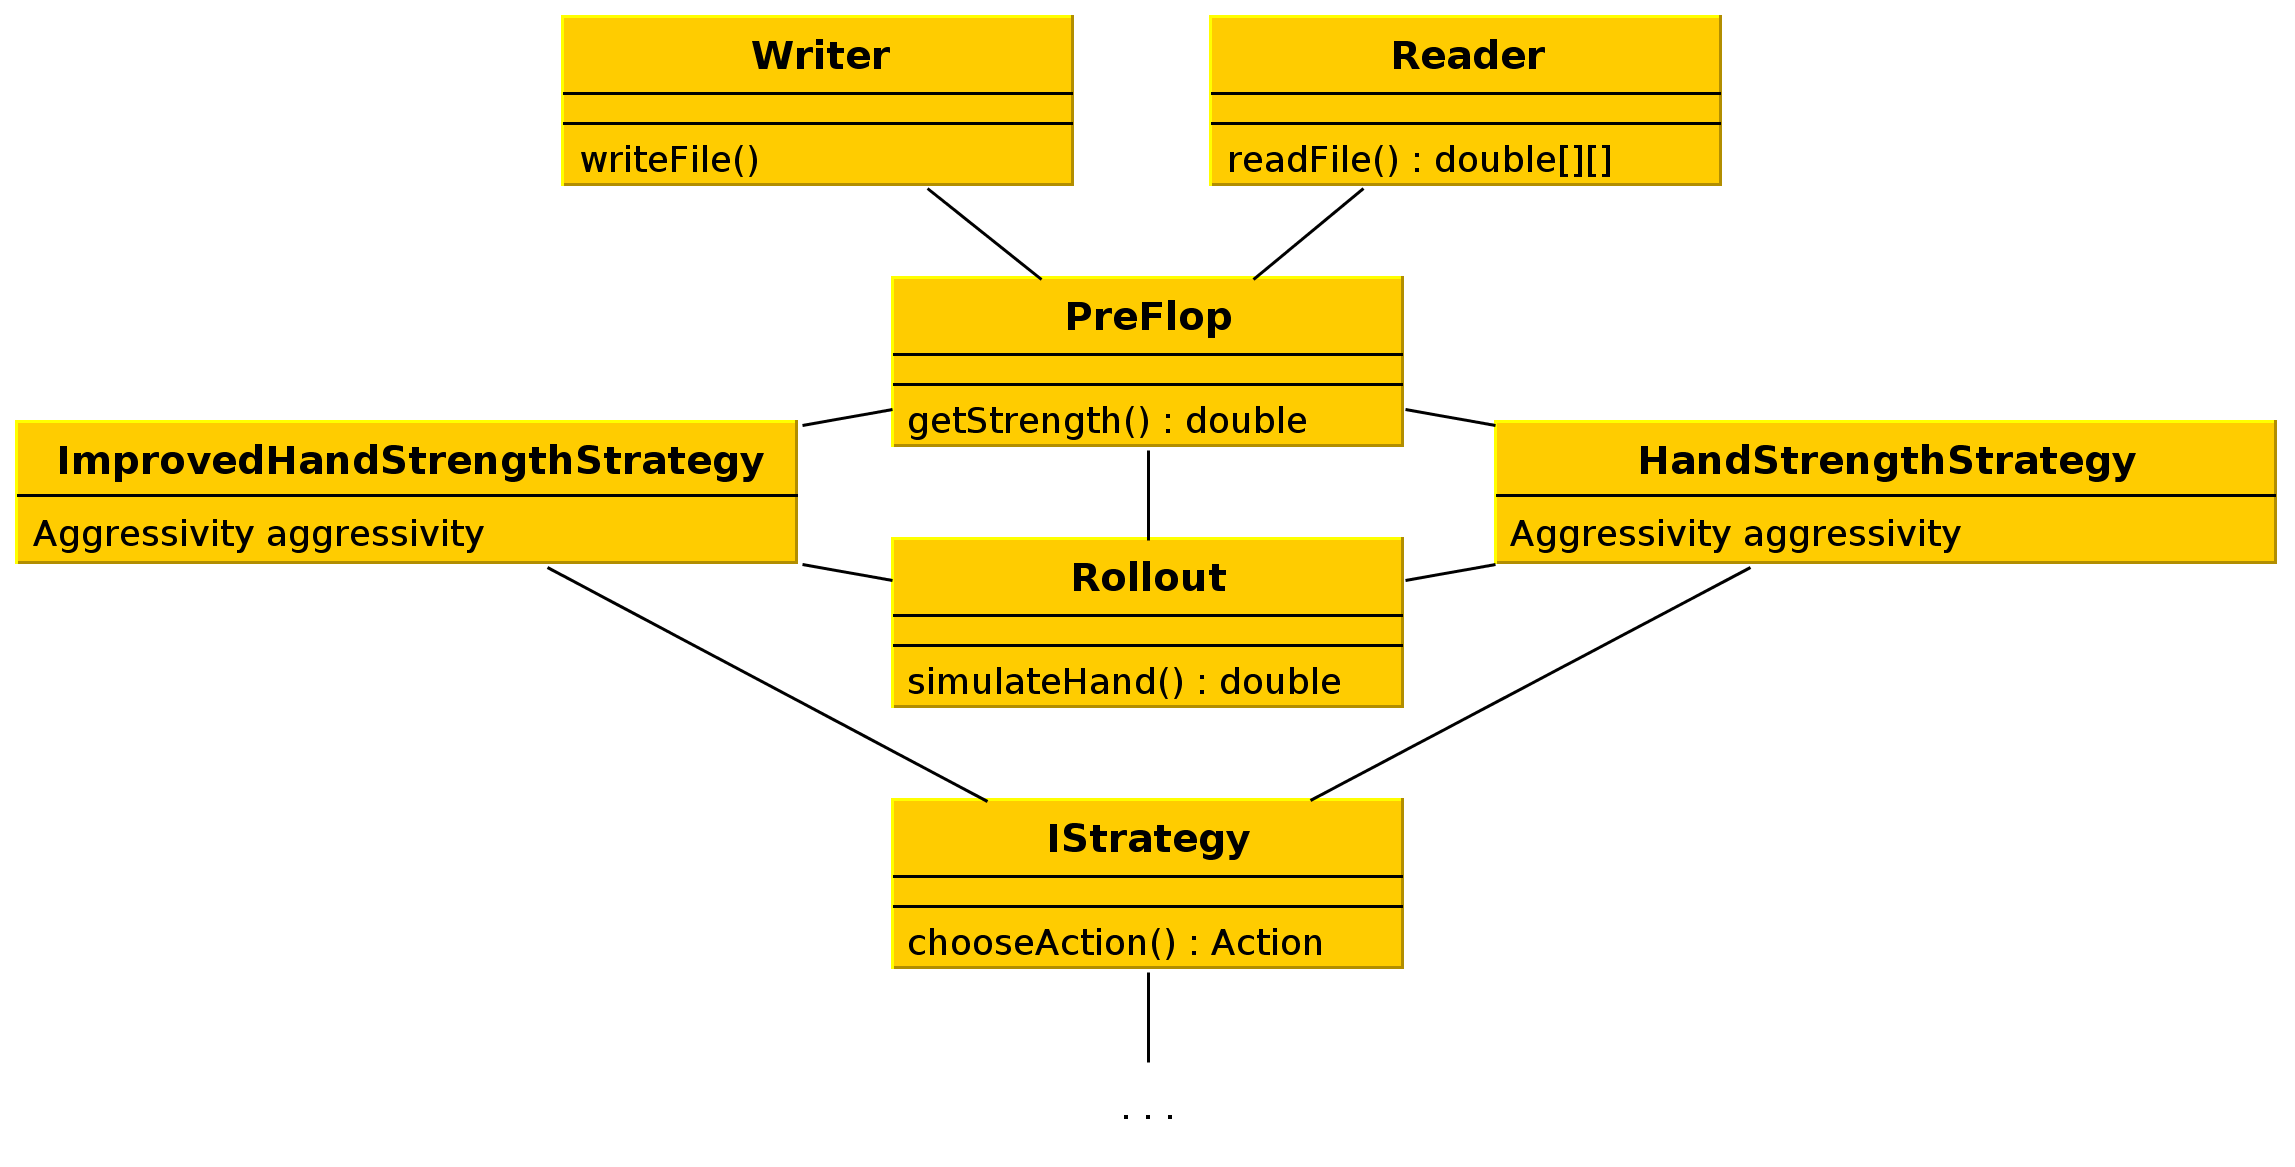
\includegraphics[width=1.0\textwidth]{images/phase2}
  \caption{Software design of phase II}
  \label{fig:phase2}
\end{figure}

\section{Rollouts}
The calculation of the hand strength is done differently depending whether it's pre flop or not, because at the pre flop there are no shared cards available.

\subsection{Pre Flop}
For the calculation of the hand strength at the pre flop two cards are fixed and the remaining 50 cards are dealt out. This is done many times. The count of the number of times that these two cards win is divided by the number of rollouts to estimate the hand strength of the two cards. 

In order to reduce the number of rollout simulations the cards are divided in equivalence classes. For example the strength of a pair of Jacks is independent of the sign. Despite of that there are 169 equivalence classes. For each of these classes 10,000 rollout simulations are performed. This has to be done for every number of players between 2 and 10. So there are over 15 millions simulations to perform. Therefore it is reasonable to do this computation offline and store them in files. The figure \ref{fig:preflop} visualizes such a file.

\begin{figure}[h]
  \centering
  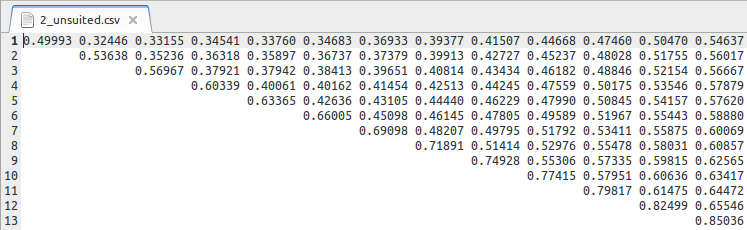
\includegraphics[width=1.0\textwidth]{images/preflop}
  \caption{Pre Flop rollout for two players and unsuited cards}
  \label{fig:preflop}
\end{figure}

\subsection{Flop, Turn and River}
After the pre flop stage there are shared cards available. Therefore the card power can be determined. Every possible combination of opposing hole cards is combined with the given shared cards to see if it yields a better hands than the own hand. This calculation is done online.

The problem with this approach is that the missing shared cards at the flop and at the turn arent't considered. Therefore the \emph{Improved Hand Strength Strategy} was implemented. Here the missing shared cards are drawn randomly out of the deck. This is done several times like at the pre flop.

\section{Strategies}
The expectation is that the phase II strategies beat the phase I strategies.

\subsection{Hand Strengh Strategy}
The amount of money the player is willing to pay $w$ is calculated on the basis of his hand strength $h$ and the aggressivity level $a$ as shown in formula \ref{equ:handStrength1}. Like in phase I the aggressivity level is a number between 1 and 3. The riskier a player the more is he willing to pay. The maximum amount the a risky player would pay is 

\begin{equation}
	\label{equ:handStrength1}
	w = e^{(h * 3 - 3)} * 100 * a + b
\end{equation}

After $w$ is calculated the player's action is detemined on the basis of $w$. If $w$ is smaller than the pot odds multiplied by the amount a call would cost the player folds. That means, that if the player hasn't to pay much (relatively to the pot size) to stay in the game he will pay at least the call. To raise $w$ has to fulfill the following condition \ref{equ:raiseCondition1} where $c$ is the cost of the call and $r$ the number of raises. The more raises there have been, the more likely the player will raise. That's because the player is sure not to frighten away the competitors knowing that they already have raised and don't want to dump their stakes. If there are only few raises the player will more likely call to prevent others from folding.

\begin{equation}
	\label{equ:raiseCondition}
	w > \frac{c}{1 + r}
\end{equation}


\subsection{Improved Hand Strengh Strategy}
The \emph{Improved Hand Strength Strategy} computes the bets the same way like the \emph{Improved Hand Strength Strategy} but it also draws the missing shared cards at the flop and at the turn. Therefore it is significantly slower, but the calculated hand strengths are expected to be more precise.

\section{Results}
Table \ref{tbl:resultsPhase2a} shows five 10,000 hand runs where \emph{Hand Strength Strategy}-players play against each other
\begin{table}[h]
	\centering
	\begin{tabular}[h]{l|r|r|r|r|r}
		& \textbf{Game 1} & \textbf{Game 2} & \textbf{Game 3} & \textbf{Game 4} & \textbf{Game 5}\\
		\hline
		Hand Strength (risky) & -248413 & -314686 & -299379 & -256889 & -255356\\
		Hand Strength (risky) & -155327 & -151467 & -154479 & -156163 & -188908\\
		Hand Strength (moderate) & -29572 & 49987 & 91098 & 10332 & 41706\\
		Hand Strength (moderate) & 84684 & 48850 & 51756 & 63958 & 60409\\
		Hand Strength (conservative) & 200887 & 173006 & 149211 & 222864 & 198017\\
		Hand Strength (conservative) & 147595 & 194157 & 161663 & 115740 & 143957\\
	\end{tabular}
	\label{tbl:resultsPhase2a}
	\caption{Results of phase II. 10.000 hands on each run.}
\end{table}
The conservative player is the most successful one. The reason for that he is only willing to play  a hand if his cards are very good. Therefore he is more likely to win at showdown.

